%%%%%%%%%%%%%%%%%%%% author.tex %%%%%%%%%%%%%%%%%%%%%%%%%%%%%%%%%%%
%
% sample root file for your "contribution" to a contributed volume
%
% Use this file as a template for your own input.
%
%%%%%%%%%%%%%%%% Springer %%%%%%%%%%%%%%%%%%%%%%%%%%%%%%%%%%


% RECOMMENDED %%%%%%%%%%%%%%%%%%%%%%%%%%%%%%%%%%%%%%%%%%%%%%%%%%%
\documentclass[graybox]{svmult}

% choose options for [] as required from the list
% in the Reference Guide

\usepackage{mathptmx}       % selects Times Roman as basic font
\usepackage{helvet}         % selects Helvetica as sans-serif font
\usepackage{courier}        % selects Courier as typewriter font
\usepackage{type1cm}        % activate if the above 3 fonts are
                            % not available on your system
%
\usepackage{makeidx}         % allows index generation
\usepackage{graphicx}        % standard LaTeX graphics tool
                             % when including figure files
\usepackage{multicol}        % used for the two-column index
\usepackage[bottom]{footmisc}% places footnotes at page bottom

%
\usepackage{url}
\usepackage{amssymb}

% see the list of further useful packages
% in the Reference Guide

\makeindex             % used for the subject index
                       % please use the style svind.ist with
                       % your makeindex program

%%%%%%%%%%%%%%%%%%%%%%%%%%%%%%%%%%%%%%%%%%%%%%%%%%%%%%%%%%%%%%%%%%%%%%%%%%%%%%%%%%%%%%%%%

\begin{document}

\title*{Performance Evaluation Experiments of Bitcoin SV Scaling Test Network}
% Use \titlerunning{Short Title} for an abbreviated version of
% your contribution title if the original one is too long
\author{Akihiro Fujihara and Takaaki Yanagihara}
% Use \authorrunning{Short Title} for an abbreviated version of
% your contribution title if the original one is too long
\institute{Akihiro Fujihara \at Chiba Institute of Technology, 2-17-1 Tsudanuma, Narashino, Chiba 275-0016, JAPAN, \email{akihiro.fujihara@p.chibakoudai.jp}
\and Takaaki Yanagihara \at Chiba Institute of Technology, 2-17-1 Tsudanuma, Narashino, Chiba 275-0016, JAPAN, \email{s1522313qq@s.chibakoudai.jp}}
%
% Use the package "url.sty" to avoid
% problems with special characters
% used in your e-mail or web address
%
\maketitle

\abstract{
Bitcoin SV Scaling Test Network (STN) is an experimental network for testing the scalability of Bitcoin with on-chain technology. 
A large amount of transactions are always sent to the P2P network, and huge blocks are generated. 
In this study, by running our STN node, the occupancy rate of transaction processing and the split probability of the blockchain are estimated. 
As a result, the estimated occupancy rate was about 1.04 and the estimated split probability was 8.5\%.
In addition, the transaction processing performance was experimentally evaluated by sending transactions including OP\_RETURN script at a high frequency of once per minute during one week.
As a result, the estimated probability that a transaction was approved was 98\%.
It was also confirmed that the distribution of latency time until a transaction is approved follows a power-law distribution at the high tail.
From these results, analysis using the theory with priority queueing is effective even in STN. 
}


\section{Introduction}
\label{sec:intro}
The origin of blockchain is a theoretical study on distributed timestamp services for electronic documents by Haber and Stornetta in the early 1990s
\cite{HS1991,BHS1993,HS1997}.
At that time, the Internet was insufficiently developed, and it was difficult to use the proposed system in a real environment.
However, the real environment was prepared by the time that Bitcoin \cite{nakamoto} appeared in 2008, and the operation of the peer-to-peer electronic cash system started on January 3, 2009.
Since then, the system has never stopped working. 
As a result of this achievement by Bitcoin, the word ``Blockchain'' (Hereinafter abbreviated as BC) was born and it has attracted attention though it is essentially the same technology as the distributed time stamp services.
Therefore, the new idea created by Bitcoin was not BC, but Nakamoto Consensus (仲基合意), where an unspecified number of nodes participating in the network form a consensus on BC. 
Although research on consensus algorithms had been conducted before the advent of Bitcoin, Nakamoto Consensus was innovative in that it proposed a method to form consensus among unspecified number of nodes on the Internet scale by combining multiple mechanisms such as Proof of Work (PoW)\cite{DN1993,JJ1999}, longest-chain rule, and incentive mechanism.


The innovative use value of Bitcoin is in micropayments of less than one yen or cent that can be realized by making transaction fees extremely low. 
Micropayment makes it possible to collect near zero (the level at which people don't care about paying) charges from a large number of users when using various services on the Internet.
Micropayments therefore have the potential to create new decentralized economic mechanisms that have never existed before.
However, the current Bitcoin Core (BTC) \cite{btc} is not used for ordinary payments as an electronic money system, but has become a store-of-value system for speculative purposes. 
Behind this, there is a technical issue that make BTC practically difficult to perform many micropayments. 


The block size limit of BTC is 1 MB, and blocks larger than this are rejected by miners. 
The average block generation time interval for BTC is controlled to ten minutes by a difficulty adjustment algorithm. 
Therefore, the system can only approve transactions that can be recorded in a block of 1 MB at maximum every ten minutes on average. 
This means that transaction processing capacity is about 7 Transactions Per Second (TPS) at maximum, which is much slower than 56,000 TPS of VISA credit cards. 
To speed up the transaction processing capacity of a BC system, one might think it becomes better to simply increase the upper limit of block size or shorten the average block generation time interval. 
However, the larger the block size, the more time it takes to transfer and share the block to all nodes on the P2P network. 
Therefore, another block is easily generated before the previously generated block is distributed to the whole P2P network, and the probability that the BC is split increases. 
When the BC is split, the hash rate of nodes that drives block generation is fragmented and its security is degraded. 
The same problem occurs even if the average block generation time is shorter than 10 minutes. 
For these reasons, there are technical difficulties in improving the transaction processing capacity, which is called blockchain scalability problem.


Various research proposals have been made to solve the scalability problem \cite{ZHZB2020} and we are also engaged in it with some previous works \cite{Fujihara2018,Fujihara2019,Fujihara2020,YF2021a,YF2021b}.
Among them, a technique like Lightning network \cite{PD2016}, in which a large amount of transactions are executed outside BC, and only the final result is written in BC at once, is attracting attention to reduce the amount of transactions to approve. 
This called off-chain scaling technique because it avoids the scalability problem by utilizing a system outside BC. 
Off-chain technology looks good, but individual transaction processing does not remain in BC.


Bitcoin has a history of being used as an illegal transaction platform in darknet markets.
In recent years, however, many cases have been reported that managers and users of these markets have been arrested \cite{silkroad,alphabay,welcome2video}.
These arrests are based on the fact that transactions published on the BC are tamper resistant and are used as legal evidence.
From this point of view, as the off-chain technology spreads, the number of transactions that cannot be tracked and audited by the government increases, making it difficult to control illegal transactions in the darknet market and becoming a hotbed for money laundering or terrorist financing.
For this reason, considering the balance with law and ethics, it is ultimately required to solve the scalability problem by the on-chain technology to approve all transactions on BC. 


In order to solve the scalability problem with on-chain, 
BloXroute\cite{bloX} introduced the network layer called Blockchain Distribution Network for additionally connecting to the P2P network to propagate larger blocks in a shorter time. 
The effort to increase the block size limit is being experimented by Bitcoin SV (BSV) \cite{bsv} Scaling Test Network (STN) \cite{bitcoinscaling}.
The block size limit of BSV is eliminated, while that of BTC is 1 MB. 
As of May 27, 2022, the average transaction processing capacity of last 24 hours was reportedly 545 TPS, and the largest block size ever mined was 4 GB. 


This paper reports some experimental results of data analysis and performance evaluation on transaction processing in STN. 
The contribution of this paper is summarized below: 
%
\begin{itemize}
  \item Using the queueing theory, we investigate the time variation of occupancy rate on transaction processing. 
	As the result, we show that the estimated occupancy rate exceeded 1 during most of the time. 
  \item Using the function of bitcoin-cli, we estimate the BC split probability. 
	The result shows that the split probability for BTC is theoretically calculated as 2\%, while that for BSV STN is experimentally estimated as about 8.5\%.
	Using this result, it was also confirmed that the average block propagation time for BSV STN is calculated to be about 53 seconds. 
  \item We also experimentally measured the latency time until transactions containing OP\_RETURN script is approved to taken into BC by sending transactions frequently as well as once per minute on average. 
	As a result, the probability that a transaction is taken into BC is 98\%, and the latency time distribution tends to follow a power distribution with exponent 3/2, which is consistent with the theory of priority queueing. 
\end{itemize}
%




\section{Related Works}
\label{sec:rworks}

\subsection{Calculation of BC Split Probability}
\label{sec:fork}

It is known that the block generation time interval of Bitcoin follows an exponential distribution. 
%
\begin{equation}
	F(t) = P(T \le t) = \int_{0}^{t} \lambda e^{-\lambda t'} dt' = 1 - e^{-\lambda t}, \label{eq:exp}
\end{equation}
where the parameter $\lambda$ is the inverse of the average block generation time.
For Bitcoin, the average block creation time is $1 / \lambda = 10$ minutes $= 600$ seconds.


The average latency time for a block to spread to 90\% of all the nodes in the P2P network of BTC is experimentally measured as $t = \tau_{fork} \fallingdotseq 12$ seconds before Compact Block Relay is applied \cite{bloX}. 
If another block is generated before the block is spread over the whole network, BC becomes split. 
Therefore, the BC split probability of BTC can be calculated as 2\% as follows.
%
\begin{equation}
  F(\tau_{fork}) = P(T \le \tau_{fork}) = 1 - e^{-\lambda \tau_{fork}} \fallingdotseq \lambda \tau_{fork} = 12/600 = 0.02. 
\end{equation}
%



\subsection{Theory of Priority Queuing}
\label{sec:priorityqueue}

Consider a queue with priority that serves customers with high priority first. 
It is known from the analysis of priority queueing that when the occupancy rate is $0 < \rho \le1 $, the latency time of low priority customers follows a power distribution with a power exponent of $3/2$, and the tail of the distribution also has an exponential cutoff\cite{OB2005}. 
%
\begin{eqnarray}
  P(\tau) &=& \frac{A}{\tau^{3/2}} \exp(-\tau/\tau_0), \\
  \tau_0  &=& \frac{1}{\mu (1-\sqrt{\rho})^2}, \\
  \rho    &=& \lambda / \mu,
\end{eqnarray}
%
where $A$ is the normalized constant of the probability distribution, $\lambda$ is the average arrival rate of customers, and $\mu$ is the average service rate.
It has also been reported that the same power distribution is followed when the occupancy rate takes the supercritical state, \textit{i.e.}, $\rho > 1$. 
The difference from the case of $0 < \rho \le 1$ is that at a rate of $1 -1 / \rho $, lower priority customers cannot receive the service forever. 

Previous research\cite{KK2019} has shown that the latency time for a transaction to be approved in BTC can be explained by the theory of priority queueing where the priority is determined by its transaction fee.
Therefore, it is expected that the latency time distribution for a transaction to be approved in BSV STN is followed by the theory of priority queueing as well. 



\section{Bitcoin SV Scaling Test Network}
\label{sec:stn}

As an experiment field of the scalability, BSV started STN as a third test network after RegTest and Testnet. 
In testnet, the block size tends to be small because the number of transactions is small, but in STN, a large number of transactions are constantly sent from multiple nodes to make a huge block. 
Figure \ref{fig:unconfirmed_tx} shows a trend of the number of unconfirmed transactions in the STN. 
%
\begin{figure}[t]
  \vspace{-35mm}
  \begin{center}
    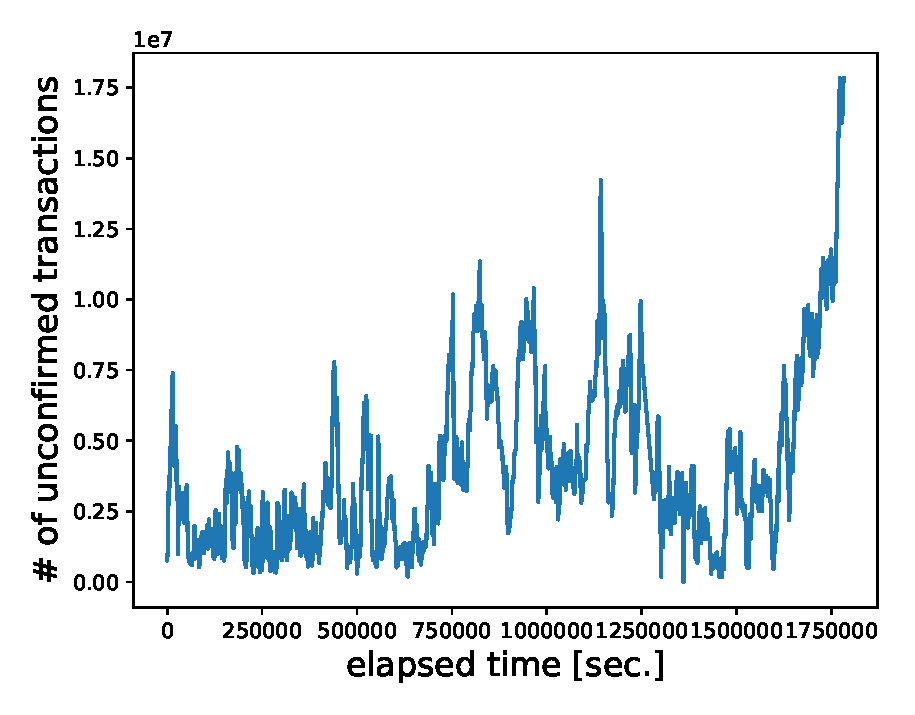
\includegraphics[width=70mm]{time_vs_tx-plot.eps}
  \end{center}
  \vspace{35mm}
  %\caption{STNの未確認取引件数の時間変化}
  \caption{Trend of unconfirmed transactions in STN.}
  \label{fig:unconfirmed_tx}
  %  \ecaption{english caption is here}
\end{figure}
%
We collected the number of unconfirmed transactions periodically from the BSV blockchain explorer named whatsonchain\cite{woc}.
Figure \ref{fig:unconfirmed_tx} shows that there are regularly more than 1 million transactions in the transaction pool. 
We can also see that the number of transactions sometimes reaches more than 10 million.


The network of STN is open to the public, and anyone can participate in the network. 
However, as system requirements for node construction, performance of 8--16 cores for CPU, 64 GB (+64 GB Swap) for memory, over 3 TB for hard disk, and over 1 Gbit for both up and down Internet connection are required.
The total size of BC was as huge as 2.4 TB at that time in February 9, 2021, while it was about 22 GB in Testnet and 284 GB in Mainnet. 
And, the block height of BC of STN became 15,216 as of February 9, 2021, and it is small, which is because BC has been reorganized several times in the past.

CPU mining is possible in STN since the difficulty varies from one to several tens.
The block mining difficulty over time is shown in Fig.~\ref{fig:difficulty}.
%
\begin{figure}[t]
  \vspace{-35mm}
  \begin{center}
    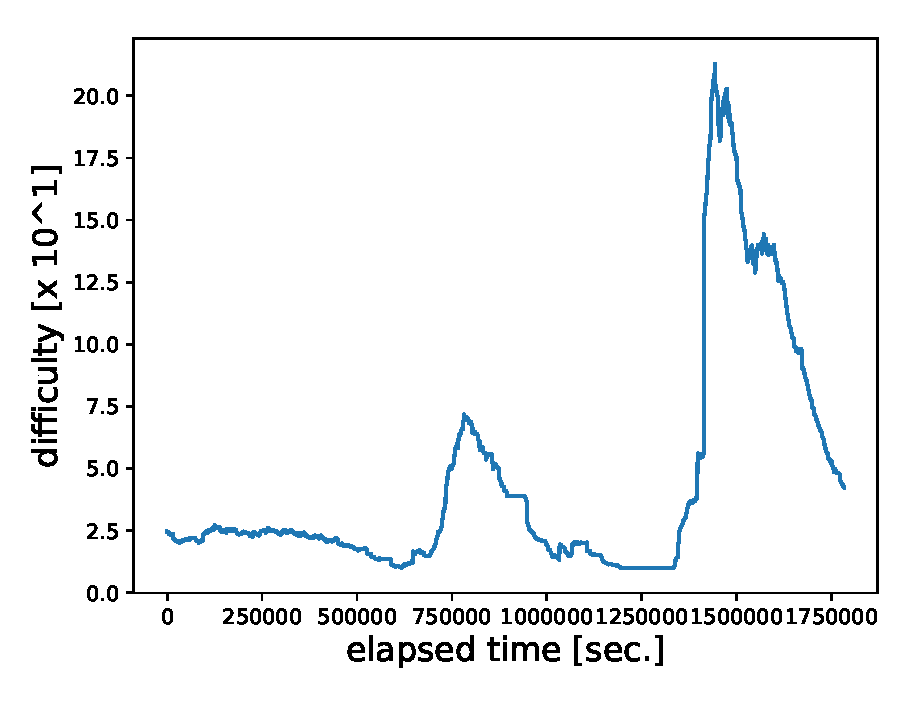
\includegraphics[width=70mm]{time_vs_difficulty-plot.eps}
  \end{center}
  \vspace{35mm}
  %\caption{ブロック採掘の難易度の時間変化}
  \caption{Block mining difficulty over time.}
  \label{fig:difficulty}
  %  \ecaption{english caption is here}
\end{figure}
%

It is recommended that STNs be configured with a maximum block size of 10 GB and the number of Bitcoin scripts allowable in a transaction is limited to 2GB of memory.
Figures \ref{fig:block_size} show the size distribution of blocks mined so far. 
%
\begin{figure}[t]
  \vspace{-35mm}
  \begin{center}
    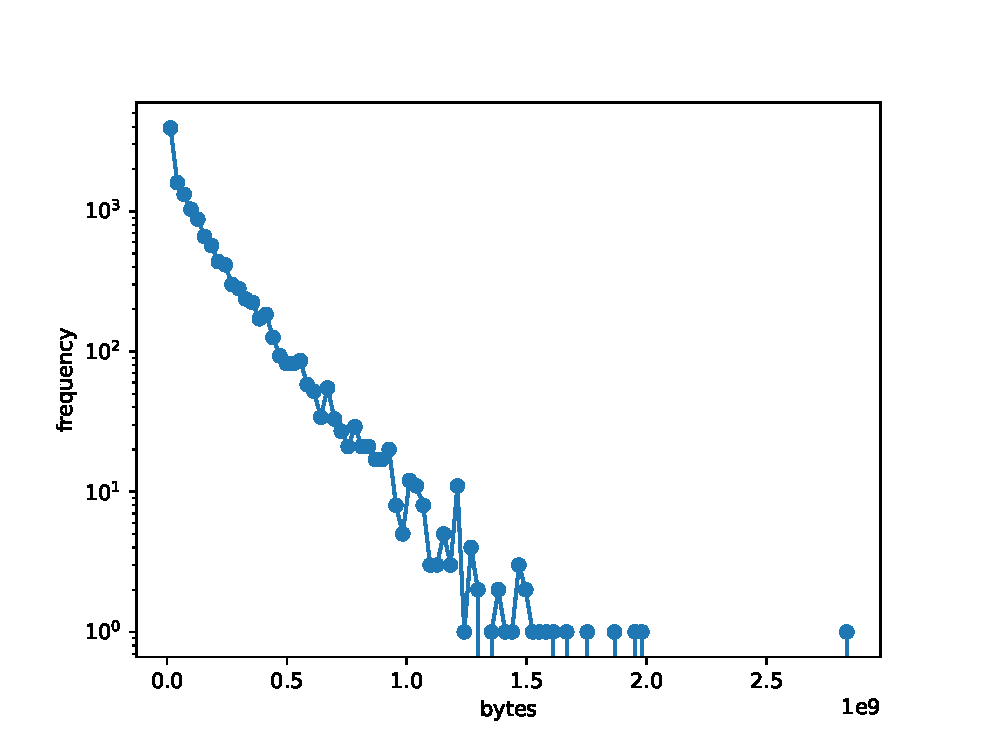
\includegraphics[width=70mm]{bsv_stn-block_bytes-semilogy2.eps}
    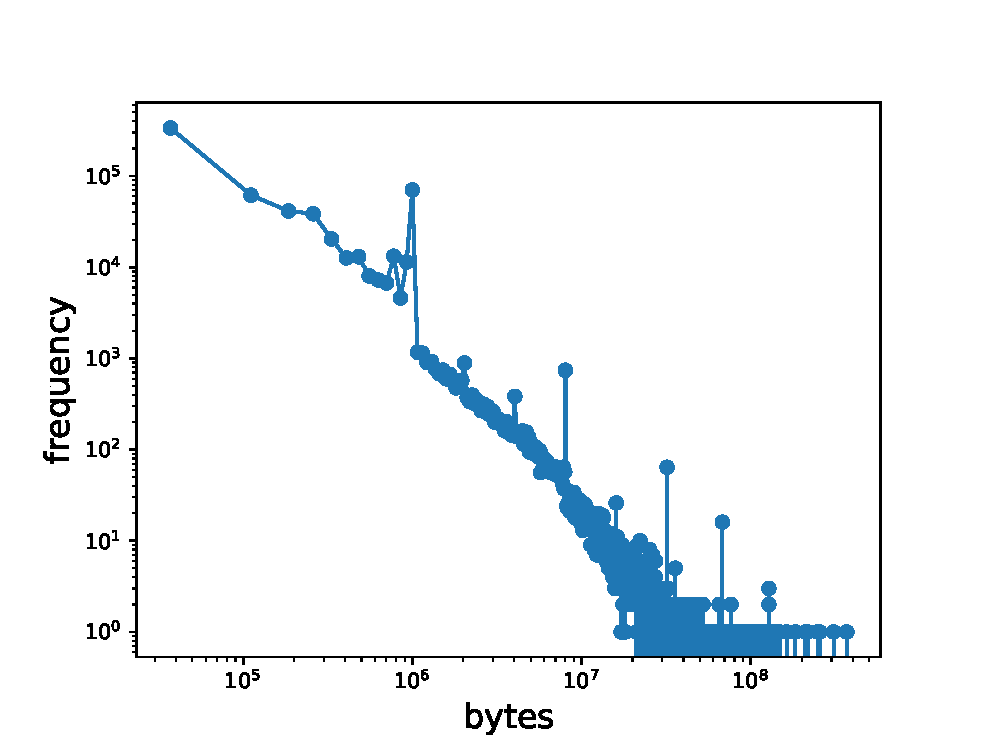
\includegraphics[width=70mm]{bsv_mainnet-block_bytes-loglog.eps}
  \end{center}
  \vspace{35mm}
  \caption{Block Size Distribution in Bitcoin SV (Above is STN, below is Mainnet).}
  \label{fig:block_size}
  %  \ecaption{english caption is here}
\end{figure}
%
The block size distribution of STN seems to follow an exponential distribution.
The largest block size ever mined was 2.9 GB.
On the other hand, the figure below in Figs.~\ref{fig:block_size} shows the block size distribution in Mainnet, which interestingly seems to follow a power distribution rather than an exponential distribution.
It also seems to obey the Pareto-Zipf law (= the power-law distribution with a power exponent 2). 
This difference in both the distributions might come from the fact that Bitcoin in Mainnet has a market value and that in STN does not, but the reason why the difference exists is not well understood. 


The BSV recommends recording the miner ID on the blocks mined to assess the reputation of the miner.
Figures \ref{fig:minerrank_stn} and \ref{fig:minerrank_mainnet} show the results of calculating the ranking of block mining frequency with reference to the miner ID.
%
\begin{figure}[t]
  \vspace{-35mm}
  \begin{center}
    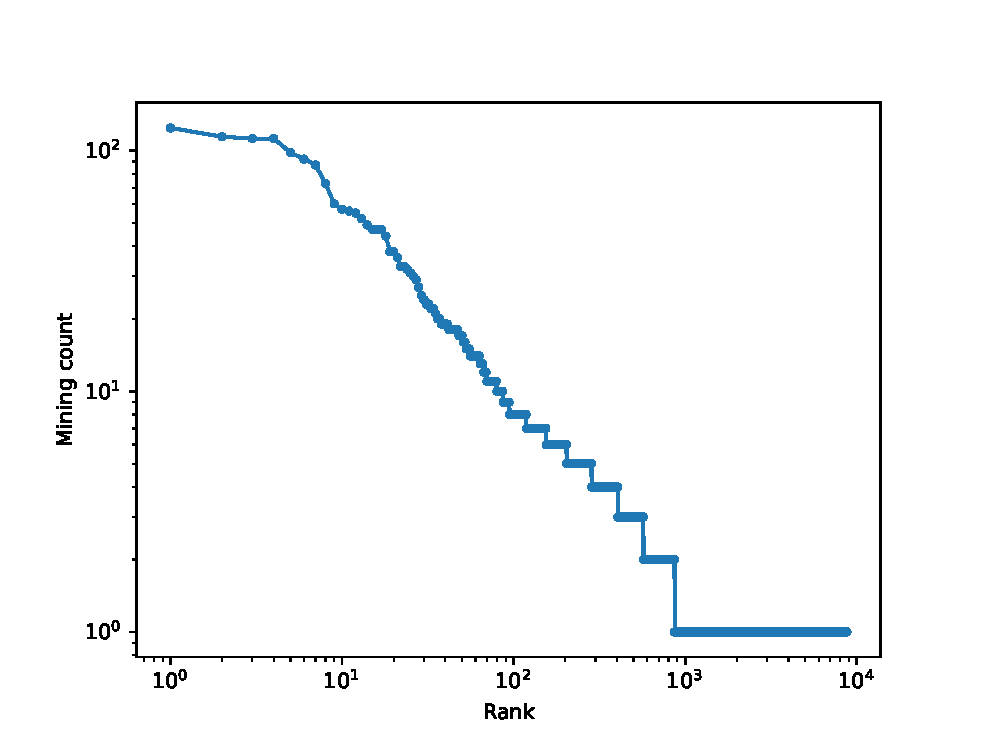
\includegraphics[width=70mm]{bsv_stn-block_miners-ranking-loglog.eps}
  \end{center}
  \vspace{35mm}
  \caption{Block mining frequency ranking calculated with reference to miner ID (STN)}
  \label{fig:minerrank_stn}
  %  \ecaption{english caption is here}
\end{figure}
%
%
\begin{figure}[t]
  %\vspace{-35mm}
  \begin{center}
    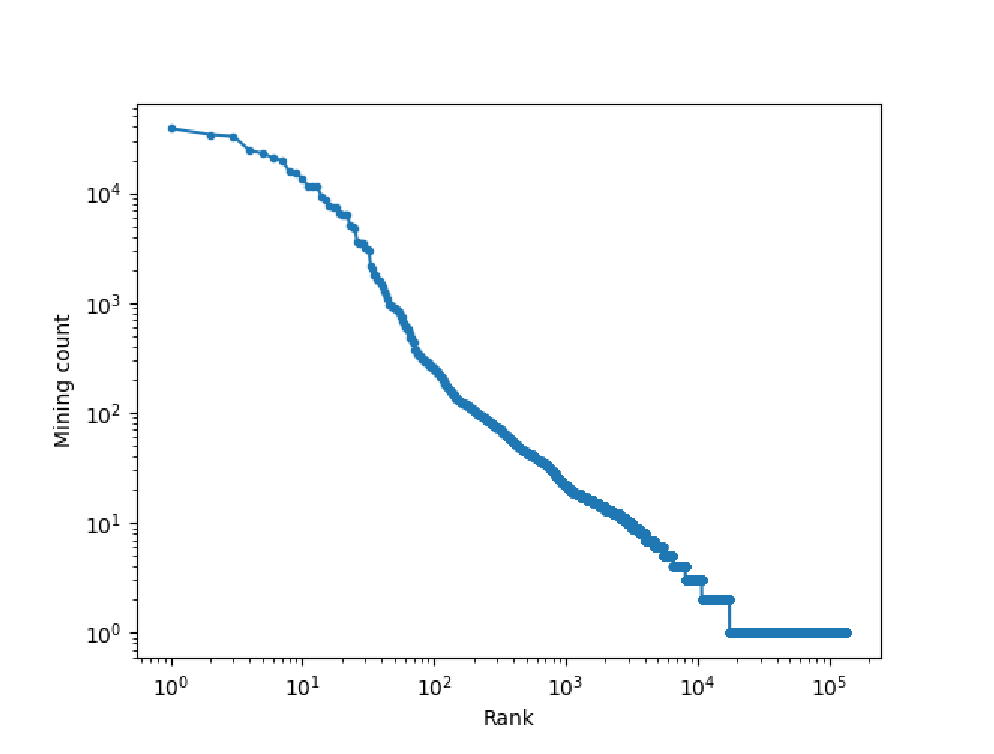
\includegraphics[width=70mm]{bsv_mainnet-block_miners-ranking-loglog.eps}
  \end{center}
  %\vspace{35mm}
  \caption{Block Mining Frequency Ranking Calculated Based on Miner ID (Mainnet)}
  \label{fig:minerrank_mainnet}
  %  \ecaption{english caption is here}
\end{figure}
%
The block mining frequency is both STN and Mainnet seem to follow a power-law distribution.



\section{Performance Evaluation Experiments}
\label{sec:experiments}

\subsection{Experiment 1: Estimating the Occupancy Rate of Approving Transactions in STN}
\label{sec:occupancyrate}

From the time variation of the number of unconfirmed transactions in Fig.~\ref{fig:unconfirmed_tx}, the occupancy rate of STN was estimated. 
Figure~\ref{fig:occupancyrate} shows the results of calculating the time variation of the estimated occupancy rate of STN $\tilde{\rho}$ based on queuing theory.
%
\begin{figure}[tb]
  \vspace{-35mm}
  \begin{center}
    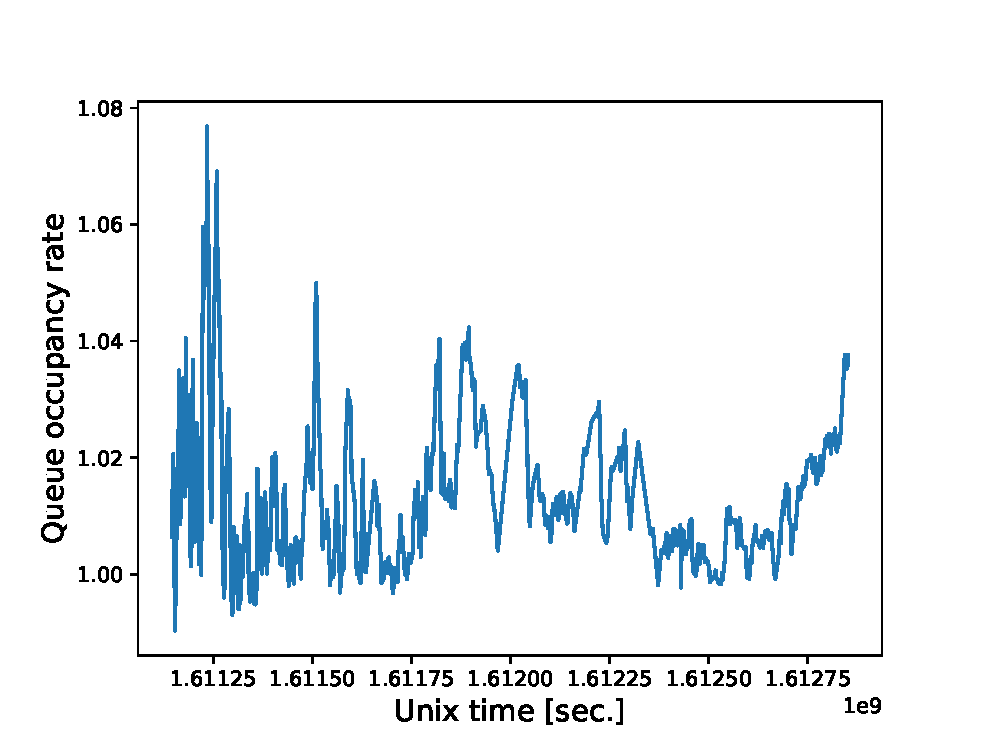
\includegraphics[width=70mm]{bsv_stn-rho-queue_occupancy_rate.eps}
  \end{center}
  \vspace{35mm}
  \caption{Time variation of the estimated occupancy rate in STN $\tilde{\rho}$.}
  \label{fig:occupancyrate}
  %  \ecaption{english caption is here}
\end{figure}
%
It is observed that the estimated occupancy rate exceeds 1 in most time periods. 
This result suggests that there are almost always unapproved transactions. 
Using collected data from November 4, 2020 to February 9, 2021, the estimated occupancy rate was calculated as $\tilde{\rho} \fallingdotseq 1.04$. 
From these results, it is considered that there is a probability of $1 -1 / \tilde{\rho} \fallingdotseq 0.0387$ that transactions are issued but not approved to be finally recorded in BC. 
The reason why transactions are not approved seems to be that STN always have a large number of unapproved transactions, but miners tend to approve transactions with high fees. So, if the fee is low, the transaction approval will be delayed and eventually forgotten because of overflows from the memory of transaction pool. 



\subsection{Experiment 2: Estimating BC Split Probability}
\label{sec:sork}

If you run an STN node, you will see that when a large block has been created, a large split of BC will occur and it will go into a safe mode where you will not be able to transfer money using the bitcoin-cli command. 
Once this large split occurs, it sometimes takes nearly half a day to resolve.
We conducted an experiment to estimate this BC split probability using warnings when running the command ``bitcoin-cli getinfo''.


During the period from November 4, 2020 to January 13, 2021, the warnings were collected once every 10 seconds. We collected them 594,880 times in total. 
As the result, we observed two kinds of warnings as follows.
%
\begin{itemize}
  \item Warning: The network does not appear to fully agree! We received
        headers of a large fork. Still waiting for block data for more details.
	(Occurred 32,724 times, approximately 5.5\% in total.)

  \item Warning: The network does not appear to fully agree! Some miners
        appear to be experiencing issues. A large valid fork has been detected. 
	(Occurred 17,782 times, approximately 3\% in total.)
\end{itemize}
%
From these results, we can estimate the BC split probability to be about $(5.5 + 3 =) 8.5$\%.
This is about four times larger than the BC split probability in BTC. 
By the way, when the split probability of BSV Mainnet was evaluated by the same method, it became 0\%.
If $F(t) = 0.085$ and $\lambda = 1/600$ are substituted in Eq.~(\ref{eq:exp}), then it derives $t = \tau_{fork} \fallingdotseq 53$ seconds, so that the average block propagation time in STN can be estimated to be about 53 seconds. 



\subsection{Experiment 3: Testing Transaction Processing Performance}
\label{sec:method}

%常に沢山の取引がTransaction poolにある状況で,取引がBCに取り込まれるまでにどの程度の時間がかかるかを実験により性能評価した.
In this paper, we experimentally evaluate how long it takes for transactions to be approved in the situation that there are always many transactions in the transaction pool. 
%実験期間を2021年1月7〜14日の1週間に設定し,期間中に分岐による取引送信ができない場合を除いて常に1分に1回の頻度で,前の1分間にFlightradar24 \cite{flightradar24} のADS-Bデータの収集ノードから千葉工業大学のある津田沼周辺を飛行する民間航空機の位置情報を収集し,OP\_RETURNスクリプトとしてデータを含めた取引の送信を行った.
Our experimental period was set for 1 week from January 7 to 14, 2021, and the location information of airplanes which flew around Tsudanuma where Chiba Institute of Technology is located was collected using ADS-B \cite{flightradar24} every one minutes. 
To do this, we wrote a program to automatically generate transactions including the collected data using OP\_RETURN script to send the P2P network. 
%1取引あたりのサイズは63KB未満になるようにした.
%また取引手数料は0.001BSVに固定した.
In the experimental settings, the data size per transaction was less than 63 KB and the transaction fee was fixed at 0.001 BSV. 
%実験結果に関するその他の詳細情報はGithub に掲載した
Additional details about the results are available on our Github website 
\footnote{\url{https://github.com/cit-fujihalab/stn_experiments}}.



%実験期間の経過時間と取引が取り込まれたブロック番号の対応関係を図\ref{fig:exp3-1}に示す.
Figure~\ref{fig:exp3-1} shows the relation between the elapsed time of the experiment period and the block number in which the transaction was approved. 
%
\begin{figure}[tb]
  %\vspace{-35mm}
  \begin{center}
    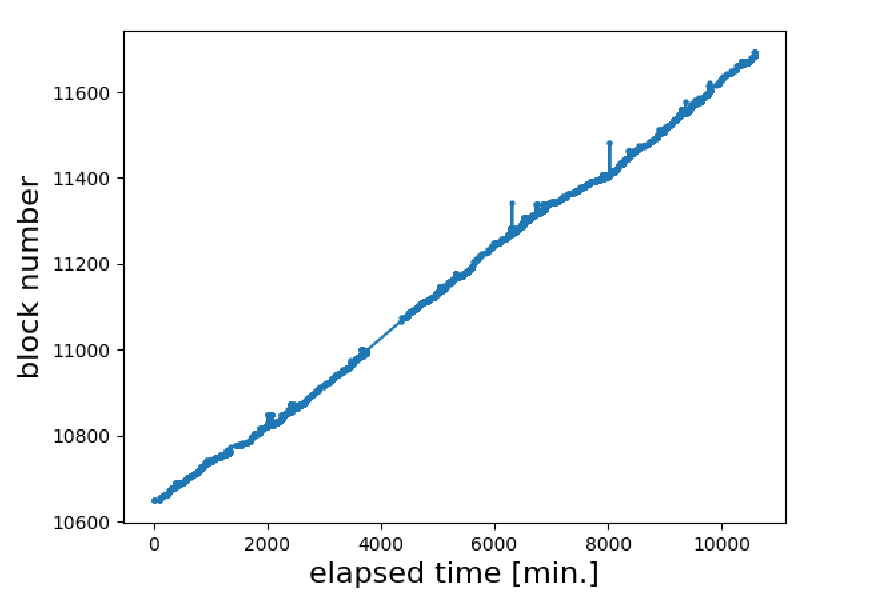
\includegraphics[width=70mm]{exp3-1.eps}
  \end{center}
  %\vspace{35mm}
  %\caption{経過時間と取引が取り込まれたブロック番号の対応関係}
  \caption{Relation between the elapsed time and the block number where the transaction was approved.}
  \label{fig:exp3-1}
  %  \ecaption{english caption is here}
\end{figure}
%
%実験期間中に合計6,828取引を送信したが,そのうち104取引はBCに取り込まれなかった.
In total, 6,828 transactions were sent during the experimental period, and 104 of them were not approved and were not recorded in BC. 
%このことより,取引がBCに取り込まれない確率が$(104/6828 \fallingdotseq) 0.02$と計算できる.
From this, the probability that the transaction is not approved can be calculated as $(104/6828 \fallingdotseq) 0.02$.
%この結果は\ref{sec:occupancyrate}節で計算した$1-1/\tilde{\rho} \fallingdotseq 0.0387$の確率でBCに取り込まれない取引が出現していると推定した結果とほぼ同じ値になっていることが確認できる.
This result is almost the same as the result calculated in Fig.~\ref{sec:occupancyrate}. 


%次に取引送信からBCに取り込まれるまでにかかる時間のヒストグラムを図\ref{fig:exp3-2}に示す.
A histogram of the latency time of the transaction to be approved is shown in Fig.~\ref{fig:exp3-2}.
%
\begin{figure}[t]
  %\vspace{-35mm}
  \begin{center}
    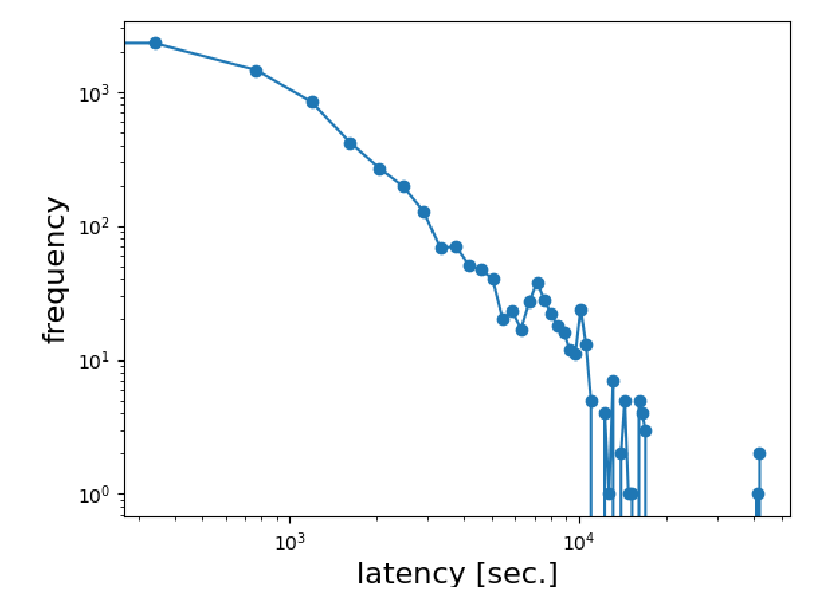
\includegraphics[width=70mm]{exp3-2.eps}
  \end{center}
  %\vspace{35mm}
  %\caption{取引送信からBCに取り込まれるまでにかかる時間のヒストグラム}
  \caption{Histogram of latency time of transaction to be approved.}
  \label{fig:exp3-2}
  %  \ecaption{english caption is here}
\end{figure}
%
%ブロック生成時間分布が指数分布に従うことから,半日程度の短期間ではBCに取り込まれる時間は指数分布に従うが,1週間程度の長期間になると指数分布から外れてくる.
Since the distribution of block generation time interval follows the exponential distribution, the latency time also follows the exponential distribution in the short term which are about half a day, but it deviates from the exponential distribution in the long term which are about one week.
%実際に図\ref{fig:exp3-2}のとおり両対数プロットで直線的な傾向が現れる為,冪分布に従う傾向が現れていることが確認できる.
In fact, as shown in Fig.~\ref{fig:exp3-2}, a linear trend appears in the double-logarithmic plot, which means that it follows the power-law distribution.
%また冪指数を両対数プロットの傾きから見積もると3/2に近いことが分かる.
The power index can be estimated from the slope of the double-logarithm plot and is close to 3/2.
%これらの結果は優先権付き待ち行列の理論解析結果と矛盾しない.
These results are consistent with the theoretical analysis of priority queueing.
%このことから手数料の低い取引が優先度が低くなり,BCに取り込まれるまでに時間がかかっていることが予想される.
This indicates that the transaction with low fee becomes low priority, and it takes more time to be approved than that with high fee. 



%取引サイズに対する取引手数料の割合と取引がBCに取り込まれるまでにかかった時間の関係を図\ref{fig:exp3-3}に示す.
Figure \ref{fig:exp3-3} shows the relation between the fee rate (= the ratio of transaction fee per byte of transaction) and the latency time until the transaction is approved. 
%
\begin{figure}[t]
  %\vspace{-35mm}
  \begin{center}
    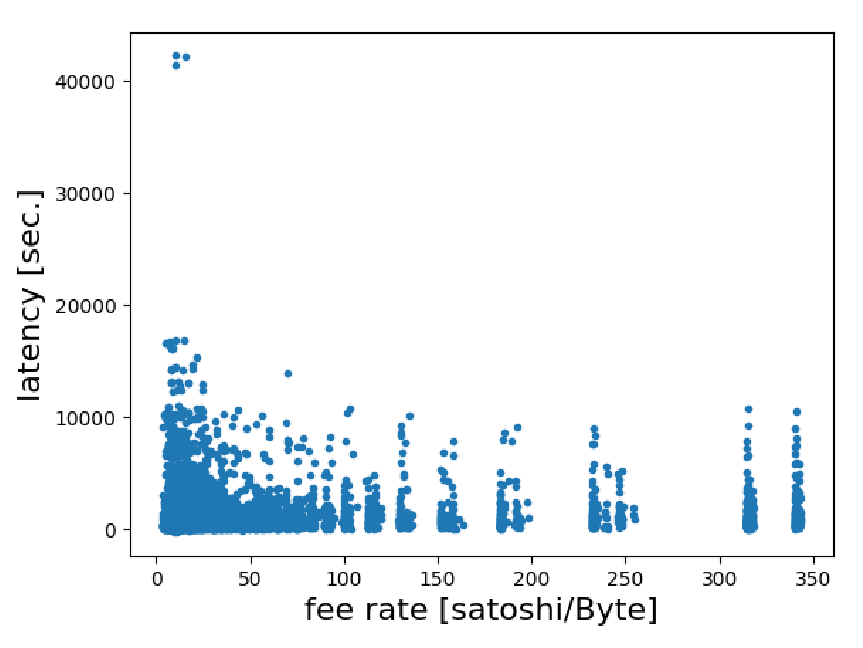
\includegraphics[width=70mm]{exp3-3.eps}
  \end{center}
  %\vspace{35mm}
  %\caption{取引サイズに対する取引手数料の割合と取引がBCに取り込まれるまでにかかった時間の関係}
  \caption{Relation between the fee rate and the latency time until the transaction is approved.}
  \label{fig:exp3-3}
  %  \ecaption{english caption is here}
\end{figure}
%
%割合(fee rate)が低いとBCに取引が取り込まれるまでに時間がかかっていることが分かる.
A low fee rate indicates that it is taking a long time for transactions to be incorporated into BC.
%このことからSTNにおいても優先権付き待ち行列理論による考察は有効であると考えられる.
From the above results, we conclude that it is also effective for STN to be analyzed using the theory of priority queueing as well as BTC. 



\section{Conclusion}
\label{sec:conclusion}

%本研究ではBitcoin STNのノードを構築し,ブロックサイズの上限を撤廃した環境における取引処理に関するデータ分析や性能評価実験を行った.
In this study, we conducted data analysis and performance evaluation of Bitcoin SV STN where the upper limit of block size is removed. 
%取引処理の稼働率の時間変化を調べた結果,推定稼働率は殆どの時間帯において1を超えていることが分かった.
As a result of examining the time variation of the occupancy rate of transaction processing capacity, we showed that the estimated occupancy rate almost always exceeded one. 
%bitcoin-cliの機能を用いてBCの分岐確率の推定も行った結果,STNでは約8.5\%となり,BTCの4倍超の確率となっていることが分かった.
Using the command ``bitcoin-cli getinfo'', we estimated the BC split probability. 
We showed that the probaiblity for STN is about 8.5\%, which is more than 4 times larger than that for BTC.
%またP2Pネットワークの平均ブロック転送時間も約53秒と推定できた.
The average block propagation time of the P2P network was also estimated to be about 53 seconds.
%OP\_RETURNスクリプトを含む取引を1分に1回の高頻度で1週間の期間,転送することで取引処理性能を実験的に評価した.
The performance of transaction processing was also experimentally evaluated by transferring transactions containing OP\_RETURN scripts at a high frequency of once per minute during one week.
%その結果,取引がBCに取り込まれる確率は98\%であり,その時間分布は長期的には冪分布に従うような傾向が確認できた.
As a result, it was found that the probability of transactions being approved was 98\%, and the latency time follows the power-law distribution in the long term. 
%また優先権付き待ち行列の理論と矛盾しない3/2の冪指数に従う傾向も確認できた.
We also confirmed that the power index is about 3/2, which is consistent with the theory of priority queueing.
%このことからSTNにおいても優先権付き待ち行列理論による考察は有効であると言える.
From these results, we concluded that the theory with priority queueing is effective to analyze STN. 



\begin{acknowledgement}
 This work was partially supported by the Japan Society for the Promotion of 
Science (JSPS) through KAKENHI (Grants-in-Aid for Scientific Research) Grant 
Number 20K11797. 
\end{acknowledgement}



%%
%\section*{Appendix}
%\addcontentsline{toc}{section}{Appendix}
%%
%%




\begin{thebibliography}{99}

% Blockchain
\bibitem{HS1991}
  S. Haber and W. S. Stornetta, 
  ``How To Time-Stamp a Digital Document,''
  J. Cryptology, 3, 99-111 (1991)
  %\url{https://link.springer.com/content/pdf/10.1007\%2FBF00196791.pdf}

\bibitem{BHS1993}
  D. Bayer, S. Haber, and W. S. Stornetta,
  ``Improving the Efficiency and Reliability of Digital Time-Stamping,''
  Sequences II: Methods in Communication, Security, and Computer Science, 
  pp. 329-334 (1993).

\bibitem{HS1997}
  S. Haber and W. S. Stornetta, 
  ``Secure Names for Bit-Strings,''
  CCS'97: Proceedings of the 4th ACM conference on Computer and 
  communications security, pp. 28-35 (1997).
  %\url{https://nakamotoinstitute.org/static/docs/secure-names-bit-strings.pdf}


% Bitcoin
\bibitem{nakamoto}
  S. Nakamoto, 
  ``Bitcoin: A Peer-to-Peer Electronic Cash System''
  (White paper), 2008 
  \url{https://bitcoin.org/bitcoin.pdf}
  \url{https://www.bitcoinsv.io/bitcoin.pdf}


% Proof of Work
\bibitem{DN1993}
  C. Dwork and M. Naor, 
  ``Pricing via Processing or Combating Junk Mail,''
  Advances in Cryptology (CRYPTO'92), 
  Lecture Notes in Computer Science, vol. 740, Springer (1993). 
  %\url{https://web.cs.dal.ca/~abrodsky/7301/readings/DwNa93.pdf}


\bibitem{JJ1999}
  M. Jakobsson and A. Juels, 
  ``Proofs of Work and Bread Pudding Protocols (Extended Abstract),''
  In: Preneel B. (eds) Secure Information Networks, 
  The International Federation for Information Processing, 
  vol 23, Springer (1999).
  %\url{https://www.arijuels.com/wp-content/uploads/2013/09/PoW.pdf}


\bibitem{btc}
  Bitcoin Core 
  \url{https://github.com/bitcoin/bitcoin}


% scalability problem
\bibitem{ZHZB2020}
  Q. Zhou, \textit{et al.}, 
  ``Solutions to Scalability of Blockchain: A Survey''
  IEEE Access, Vol. 8, pp.16440-16455, IEEE, 2020. 


\bibitem{Fujihara2018}
  A. Fujihara,
  ``Proposing a System for Collaborative Traffic Information Gathering and 
  Sharing Incentivized by Blockchain Technology,''
  The 10th International Conference on Intelligent Networking and 
  Collaborative Systems (INCoS-2018), pp.170-182 (2018)
  \url{https://link.springer.com/chapter/10.1007/978-3-319-98557-2_16}

\bibitem{Fujihara2019}
  A. Fujihara,
  ``PoWaP: Proof of Work at Proximity for a crowdsensing system for 
  collaborative traffic information gathering,'' 
  Internet of Things, 100046, Elsevier (2019).
  \url{https://www.sciencedirect.com/science/article/pii/S254266051830177X}

\bibitem{Fujihara2020}
  A. Fujihara, 
  ``Proposing a Blockchain-Based Open Data Platform and Its Decentralized Oracle,''
  Advances in Intelligent Networking and Collaborative Systems (INCoS2019), 
  Advances in Intelligent Systems and Computing, 
  Vol. 1035, pp. 190--201, Springer (2020).
  \url{https://link.springer.com/chapter/10.1007/978-3-030-29035-1_19}

\bibitem{YF2021a}
  T. Yanagihara and A. Fujihara, 
  ``Considering Cross-Referencing Method for Scalable Public Blockchain,''
  Advances in Internet, Data and Web Technologies, 
  Lecture Notes on Data Engineering and Communications Technologies, 
  Vol. 65, pp. 220-231, Springer (2021). 
  \url{https://link.springer.com/chapter/10.1007/978-3-030-70639-5_21}

\bibitem{YF2021b}
  T. Yanagihara and A. Fujihara,
  ``Cross-Referencing Method for Scalable Public Blockchain,''
  Internet of Things, Vol. 15, 100419 (2021). 
  \url{https://www.sciencedirect.com/science/article/pii/S2542660521000639}


\bibitem{PD2016}
  J. Poon and T. Dryja, 
  ``The Bitcoin Lightning Network: Scalable Off-Chain Instant Payments,'' 
  (2016) \url{https://lightning.network/lightning-network-paper.pdf}


\bibitem{silkroad}
  FBI, 
  ``Manhattan U.S. Attorney Announces Seizure of Additional \$28 Million 
    Worth of Bitcoins Belonging to Ross William Ulbricht, Alleged Owner 
    and Operator of ``Silk Road'' Website, '' 2013.
  \url{https://archives.fbi.gov/archives/newyork/press-releases/2013/manhattan-u.s.-attorney-announces-seizure-of-additional-28-million-worth-of}\\
  \url{-bitcoins-belonging-to-ross-william-ulbricht-alleged-owner-and}\\
  \url{-operator-of-silk-road-website}

\bibitem{alphabay}
  The US Department of Justice,
  ``AlphaBay, the Largest Online 'Dark Market,' Shut Down,'' 2017.
  \url{https://www.justice.gov/opa/pr/alphabay-largest-online-dark-market-shut-down}

\bibitem{welcome2video}
  The US Department of Justice,
  ``South Korean National and Hundreds of Others Charged Worldwide in the Takedown 
    of the Largest Darknet Child Pornography Website, Which was Funded by Bitcoin,'' 
  2019.
  \url{https://www.justice.gov/opa/pr/south-korean-national-and-hundreds-others-charged-worldwide}\\
  \url{-takedown-largest-darknet-child}



\bibitem{bloX}
  U. Klarman, \textit{et al.},
  ``bloXroute: A Scalable Trustless Blockchain Distribution Network''
  (White paper), 2018.
  \url{https://bloxroute.com/wp-content/uploads/2018/03/bloXroute-whitepaper.pdf}


\bibitem{bsv}
  Bitcoin SV (Satoshi Vision) 
  \url{https://github.com/bitcoin-sv/bitcoin-sv}

\bibitem{bitcoinscaling}
  Bitcoin Scaling Test Network
  \url{https://bitcoinscaling.io/}




\bibitem{OB2005}
  J. G. Oliveira and A.-L. Barab\'asi,
  ``Darwin and Einstein correspondence patterns,'' 
  Nature 437, 1251, 2005.


\bibitem{KK2019}
  S. Kasahara and J. Kawahara,
  ``Effect of Bitcoin fee on transaction-confirmation process,''
  Journal of Industrial and Management Optimization, 15 (1): 365-386, 2019.


\bibitem{woc}
  WhatsOnChain.com, BSV Explorer - STN,
  \url{https://stn.whatsonchain.com/}



% Flightradar24
\bibitem{flightradar24}
  Flight Tracker | Flightradar24 | Track Planes in Real-time,
  \url{https://www.flightradar24.com/}



\end{thebibliography}

\end{document}
